% !TeX spellcheck = en_US
% !TeX spellcheck = en_US
\RequirePackage[l2tabu, orthodox]{nag}

\documentclass[
a4paper,    
% draft,       %% produce only a draft version (mark lines that need manual edition and don't show graphics)
bibliography=totoc, % add bibilography to table of contents
11pt,         %% set default font size to 11 point
DIV=14, % replace this with a larger number to get less padding around all text (or use calc for the ideal border)
parskip=half, % how much space between paragraphs. If you prefer indention instead of space between paragraphs remove it
oneside, % replace with twoside before printing
%draft, % uncomment for faster compilation
british, % language of the document
%appendixprefix=true % in case you want Appendix A written in front of appendix headings
]{scrbook}



%--------------------------- Important Packages --------------------------------

%\usepackage[ngerman]{babel}
\usepackage[american]{babel}

% required for proper characters
\usepackage[utf8]{inputenc}
\usepackage[T1]{fontenc}


% helps with equations
\usepackage{amsmath,amssymb,amstext}
\usepackage{amsthm}


\usepackage{microtype} %slightly changes letter spacing to make text fit better

\usepackage{aas_macros} % this imports the aas_macros.sty file that is required to print bibtex exported from ADS

\usepackage[svgnames]{xcolor} % allows defining colors

%------------------------------- Helpful Features ---------------------------------

% properly format 
\usepackage{siunitx}
\DeclareSIUnit{\nothing}{\relax}
\sisetup{
	per-mode=fraction, % create a fraction instead of km h^-1
%	locale=DE,
	locale=US,
	output-decimal-marker = {.}, % useful even for German
	separate-uncertainty = true,
	quotient-mode=fraction
}

%\usepackage{nicefrac}
\usepackage[autostyle=true]{csquotes} % automatically create nice quotes with \enquote{text}
\usepackage{pdflscape}  
%\usepackage{cancel}  % In case you want to cancel out some values in an equation
\usepackage{physics} % lots of shortcuts for physics equations (e.g. $\dv{a}$)

\usepackage{subcaption} % allows to nicely put two images next to each other
\usepackage{tabularx}
\usepackage{booktabs} % nicer table seperations
\usepackage{todonotes}
%----------------------------------- Style decisions -----------------------------------

\hyphenpenalty=750 % break less words than default - try different values for success
\interfootnotelinepenalty=10000 % splitting footnotes between pages is really ugly and should only be done if really necessary 
\usepackage[sc]{mathpazo} % use the Palatino font and a fitting math font

\pagestyle{headings} 
% how the header of the pages looks like
% for something nicer take a look at fancyhdr

% xcolor is already defined above

% not sure what these two do, but they definitly do something
\colorlet{bluebookmarks}{blue}
\colorlet{blueallcolors}{blue}

%----------------------------------- Bibliography ----------------------------------------


\PassOptionsToPackage{hyphens}{url}\usepackage[
	backend=biber,
	style=authoryear-comp, % choose a style from https://de.overleaf.com/learn/latex/Biblatex_citation_styles
	%sortlocale=de_AT,
	sortlocale=en_GB,
	backref=true % use if you like it -- puts a link to the page where it is cited into the bibliography
]{biblatex}

\addbibresource{bibliographie.bib}


%---------------------------------- Source Code -----------------------------------------

\usepackage[scaled=.9]{FiraMono}
\usepackage{listings}
\usepackage{scrhack} % should fix warning
\definecolor{strings}{HTML}{008000}
\definecolor{keywords}{HTML}{000080}
\definecolor{mygray}{rgb}{0.58,0,0.82}

\lstset{ %
	%	backgroundcolor=\color{white},   % choose the background color; you must add \usepackage{color} or \usepackage{xcolor}; should come as last argument
	basicstyle=\footnotesize\ttfamily,        % the size of the fonts that are used for the code
	basewidth=0.5em,
	breakatwhitespace=false,         % sets if automatic breaks should only happen at whitespace
	breaklines=true,                 % sets automatic line breaking
	captionpos=b,                    % sets the caption-position to bottom
	%	commentstyle=\color{mygreen},    % comment style
	deletekeywords={...},            % if you want to delete keywords from the given language
	escapeinside={(*}{*)},          % if you want to add LaTeX within your code
	extendedchars=true,              % lets you use non-ASCII characters; for 8-bits encodings only, does not work with UTF-8
	frame=single,	                   % adds a frame around the code
	keepspaces=true,                 % keeps spaces in text, useful for keeping indentation of code (possibly needs columns=flexible)
	keywordstyle=\color{keywords},       % keyword style
	morekeywords={*,...},            % if you want to add more keywords to the set
	numbers=none,                    % where to put the line-numbers; possible values are (none, left, right)
	numbersep=5pt,                   % how far the line-numbers are from the code
	rulecolor=\color{black},         % if not set, the frame-color may be changed on line-breaks within not-black text (e.g. comments (green here))
	showspaces=false,                % show spaces everywhere adding particular underscores; it overrides 'showstringspaces'
	showstringspaces=false,          % underline spaces within strings only
	showtabs=false,                  % show tabs within strings adding particular underscores
	stepnumber=1,                    % the step between two line-numbers. If it's 1, each line will be numbered
	stringstyle=\color{strings},     % string literal style
	tabsize=2,	                   % sets default tabsize to 2 spaces
	language=bash
}
\lstset{literate=% support Umlauts in listings
	{Ö}{{\"O}}1
	{Ä}{{\"A}}1
	{Ü}{{\"U}}1
	{ß}{{\ss}}1
	{ü}{{\"u}}1
	{ä}{{\"a}}1
	{ö}{{\"o}}1
}


%--------------------------------------- PDF output and hyperlinks ----------------------------


\usepackage{graphicx} % support graphics

\pdfcompresslevel=9 % create small files (I think it is by default when using hyperref)
\pdfsuppresswarningpagegroup=1 % https://tex.stackexchange.com/a/78020/66733


% support hyperlinks in the PDF

\usepackage[ %
colorlinks=false,   %% turn on colored links (true is better for on-screen reading, false is better for printout versions)
linkcolor = blue,
allcolors=blue,
%%% PDF-specific display options
bookmarks=true,          %% if true, generate PDF bookmarks (requires two passes of pdflatex)
bookmarksopen=false,     %% if true, show all PDF bookmarks expanded
bookmarksnumbered=false, %% if true, add the section numbers to the bookmarks
%pdfstartpage={1},        %% determines, on which page the PDF file is opened
%  pdfpagemode=None         %% None, UseOutlines (=show bookmarks), UseThumbs (show thumbnails), FullScreen
draft=false
]{hyperref}






\hypersetup{
	pdftitle={Interpolated water retention after two-body collisions using Neural Networks and linear interpolation methods},
	pdfauthor={Lukas Winkler}
}
\title{Interpolated water retention after two-body collisions using Neural Networks and linear interpolation methods}
\subtitle{bla bla}
\author{Lukas Winkler\footnote{\texttt{a01505981@unet.univie.ac.at}}}
%\publishers{TEST}
\date{1. September 2019}

\begin{document}

	
\maketitle

\tableofcontents

% !TeX spellcheck = en_US

\addchap{Abstract}


Quos est voluptatem officiis animi et aliquid natus deserunt ad omnis perspiciatis voluptatum quas non natus sint molestiae minima officiis porro dolorem temporibus est non porro aut velit corrupti nostrum numquam facilis cupiditate esse sit quibusdam autem eum non dolores eum at in necessitatibus aliquid rerum voluptatum necessitatibus aut officia voluptates consequatur voluptatem nobis corporis quod nostrum et tempore placeat minima corrupti.

Autem animi consequatur delectus mollitia. Earum nesciunt distinctio et quam nam libero. Illum deserunt non voluptatem. Dolores quas qui aspernatur maxime reprehenderit repellat porro aliquam.%

{\let\clearpage\relax \chapter{Introduction}\label{introduction}}

One important question for planet formation is, how water got to the earth. The part of the protoplanetary disk closest to the sun was too hot to make it possible that water can condense on Earth during formation. And while there are theories that the region where ice is possible inside the snow-line moved during Earth's formation\footcite{snowline}, the most popular theory is that water moved inwards in the solar system through collisions of water-rich proto-planets.%
\todo{citation needed}


%\section{The perfect merging assumption}

To better understand how this process works, large n-body simulations over the lifetime of the solar systems have been conducted\footnote{for example \cite{dvorakSimulation}}. Most of these neglect the physical details of collisions when two bodies collide for simplicity and instead assume that a perfect merging occurs. So the entire mass of the two progenitor bodies and especially all of their water (ice) is retained in the newly created body. Obviously this is a simplification as in real collisions perfect merging is very rare and most of the time either partial accretion or a hit-and-run encounter occurs.\footcite{CollisionTypes} Therefore, the amount of water retained after collisions is consistently overestimated in these simulations. Depending on the parameters like impact angle and velocity, a large fraction of mass and water can be lost during collisions.\footcite{MaindlSummary}

%\section{Some other heading}
%\todo{find a name for this heading}

To understand how exactly the water transport works, one has to find an estimation of the mass and water fractions that are retained during two-body simulations depending on the parameters of the impact.
First, I will be shortly describing the simulation setup, the important parameters and the post-processing of the results (Chapter \ref{chapter:simulations}). Next I will summarize the results of the simulations and their properties (Chapter \ref{chapter:results}). In the main section I will then be describing three different approaches to interpolate and generalize these results for arbitrary collisions (Chapter \ref{chapter:interpolations}). 


% !TeX spellcheck = en_US
\chapter{Simulations}
\label{chapter:simulations}
\section{Model}

For a realistic model of two gravitationally colliding bodies the smooth particle hydrodynamics (\texttt{SPH}) code \texttt{miluphCUDA} as explained in \cite{Schaefer2016} and \cite{miluphaCode} is used. It is able to simulate brittle failure and the interaction between multiple materials. 

In the simulation two celestial bodies are placed far enough apart so that tidal forces can affect the collision (5 times the sum of the radii). Both objects consist of a core with the physical properties of basalt rocks and an outer mantle made of water ice. These two-body-collisions are similar to those that happen between protoplanets or the collision that created the Earth's Moon.\footcite{dvorakMoon}

To keep the simulation time short and make it possible to do many simulations with varying parameters, 20k SPH particles are used and each simulation is run for 12 hours in which every 144~seconds the current state is saved.

\section{Parameters}
\label{sec:parameters}

Six parameters have been identified that have a major influence on the result of a two-body collision. All selected parameter ranges are inspired by the physical properties that occurred in collisions in a simulation of an early solar system.\footcite{CollisionParameters} (Table \ref{tab:first_simulation_parameters})

\subsection{Impact velocity}

The collision velocity $v_0$ is defined in units of the mutual escape velocity $v_{esc}$ of the projectile and the target.\footcite{MaindlSummary} Simulations have been made from $v_0=1$ to $v_0=5$. As one expects, a higher velocity results in a stronger collision and more and smaller fragments.
\begin{equation}
	v_{esc}=\sqrt{\frac{2G(M_p+M_t)}{r_p+r_t}}
\end{equation}

\subsection{Impact angle}

The impact angle is defined in a way that $\alpha=\ang{0}$ corresponds to a head-on collision and higher angles increase the chance of a hit-and-run encounter. The simulation parameters range from $\alpha=\ang{0}$ to $\alpha=\ang{60}$

\subsection{Target and projectile mass}

The total masses in these simulations range from about two Ceres masses (\SI{1.88e+21}{\kilogram}) to about two earth masses (\SI{1.19e+25}{\kilogram}). In addition to the total mass $m$, the mass fraction between projectile and target $\gamma$ is defined. As the whole setup is symmetrical between the two bodies, only mass fractions below and equal to one have been considered.

\subsection{Water fraction of target and projectile}

The last two parameters are the mass fraction of the ice to the total mass of each of the bodies. To keep the numbers of parameter combinations and therefore required simulations low, only \SI{10}{\percent} and \SI{20}{\percent} are simulated in the first simulation set.


\begin{table}
	\centering
	\begin{tabular}{r|SSSSS}
		$v_0$ & 1 & 1.5 & 2&3 & 5 \\
		$\alpha$ & \ang{0} & \ang{20} & \ang{40} & \ang{60} &\\
		$m$ &\SI{e21}{\kilogram} & \SI{e23}{\kilogram} & \SI{e24}{\kilogram} & \SI{e25}{\kilogram} &\\
		$\gamma$ & 0.1 & 0.5 & 1 &&\\
		water fraction target & \SI{10}{\percent} & \SI{20}{\percent} &&&\\		
		water fraction projectile & \SI{10}{\percent} & \SI{20}{\percent} &&&\\
	\end{tabular}
	\caption{parameter set of the first simulation run}
	\label{tab:first_simulation_parameters}
\end{table}

\section{Execution}\todo{think of a better title}

In the first simulation run for every parameter combination from Table \ref{tab:first_simulation_parameters} a separate simulation has been started. First, the parameters and other configuration options are written in a \mbox{\texttt{simulation.input}} text file. Afterwards the relaxation program described in \cite[24\psqq]{Burger2018} generates relaxed initial conditions for all 20k particles and saves their state to \texttt{impact.0000}. Finally, \texttt{miluphcuda} can be executed with the following arguments to simulate starting from this initial condition for 300 timesteps which each will be saved in a \texttt{impact.XXXX} file.

\begin{lstlisting}[language=bash,flexiblecolumns=false]
miluphcuda -N 20000 -I rk2_adaptive -Q 1e-4 -n 300  -a 0.5 -H -t 144.0 -f impact.0000 -m material.cfg -s -g
\end{lstlisting}

This simulation ran on the \texttt{amanki} server using a \texttt{Nvidia GTX 1080} taking about \SI{30}{\minute} per simulation as the \texttt{Nvidia GTX 1080} is the fastest consumer GPU for this simulation set in a comparison of 13 tested GPUs.\footcite{Dorninger} Of these 960 simulations, 822 succeed and were used in the analysis.


\section{Post-processing}
\label{sec:postprocessing}

After the simulation the properties of the SPH particles needs to be analyzed. To do this, the \texttt{identify\_fragments} C program by Christoph Burger (part of the post-processing tools of \texttt{miluphCUDA}) uses a friends-of-friends algorithm to group the final particles into fragments. Afterwards \texttt{calc\_aggregates} calculates the mass of the two largest fragments together with their gravitationally bound fragments and its output is written into a simple text file (\texttt{aggregates.txt}).


\section{Resimulation}
\label{sec:resimulation}

To increase the amount of available data and especially reduce the errors caused by the grid-based parameter choices (Table \ref{tab:first_simulation_parameters}), a second simulation run has been started. All source code and initial parameters have been left the same apart from the six main input parameters described above. These are set to a random value in the range listed in Table \ref{tab:resimulation-parameters} apart from the initial water fractions. As they seem to have little impact on the outcome (see Section \ref{sec:cov}), they are set to \SI{15}{\percent} to simplify the parameter space.

This way, an additional \num{553} simulations have been calculated on \texttt{Nvidia Tesla P100} graphics cards on \texttt{Google Cloud}. (Of which 100 simulations are only used for comparison in Chapter \ref{sec:comparison})

\begin{table}[hb]
	\centering
	\begin{tabular}{r|SS}
		& min&max\\\hline
		$v_0$ & 1 & 5 \\
		$\alpha$ & \ang{0} & \ang{60} \\
		$m$ &\SI{1.88e+21}{\kilogram} & \SI{1.19e+25}{\kilogram}\\
		$\gamma$ & 0.1&  1 \\
		water fraction target & \SI{15}{\percent} & \SI{15}{\percent} \\		
		water fraction projectile & \SI{15}{\percent} & \SI{15}{\percent} \\
	\end{tabular}
	\caption{parameter ranges for the resimulation}
	\label{tab:resimulation-parameters}
\end{table}


% !TeX spellcheck = en_US
\chapter{Results}

For the large set of simulations we can now extract the needed values. The output of the relaxation program (\texttt{spheres\_ini\_log}) gives us the precise values for impact angle and velocity and the exact masses of all bodies. As these values differ slightly from the parameters explained in Section \ref{sec:parameters} due to the setup of the simulation, in the following steps only the precise values are considered. From the \texttt{aggregates.txt} explained in Section \ref{sec:postprocessing} the final masses and water fractions of the two largest fragments are extracted. From these the main output considered in this analysis, the water retention of the two fragments can be calculated. 

\section{Correlations}
\label{sec:cov}
One very easy, but sometimes flawed\footnote{\todo[inline]{explain issues with pearson}} way to look at the whole dataset at once is calculating the \textit{Pearson correlation coefficient} between the input parameters and the output water fraction (Figure \ref{fig:cov}). This shows the expected result that a higher collision angle (so a more hit-and-run like collision) has a higher water retention and a higher collision speed results in far less water left on the two largest remaining fragments. In addition higher masses seem to result in less water retention. The initial water fractions of the two bodies does seem to have very little influence on the result of the simulations.

\begin{figure}
	\centering
	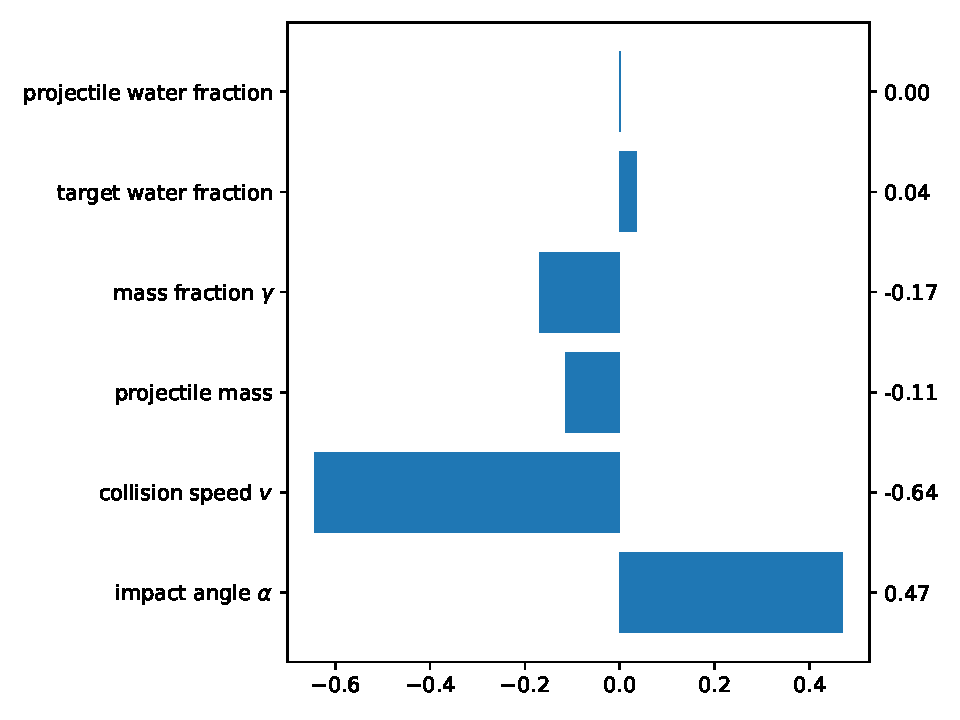
\includegraphics[width=0.8\linewidth]{images/cov.pdf}
	\caption{TODO}
	\label{fig:cov}
\end{figure}

\chapter{Interpolations}
\label{chapter:interpolations}
% !TeX spellcheck = en_US
\section{Multidimensional linear interpolation}

\subsection{Theory}

One of the easiest ways to interpolate a new value between two known values is linear interpolation. It takes the closest values and creates a linear function between them.

In one dimension, linear interpolation is pretty trivial. For example, let's assume that we have 20 random points $P$ between 0 and 1 (\textcolor{Red}{\textbullet} and  \textcolor{Blue}{\textbullet} in Figure \ref{fig:one-dim-interpolation}) and have a new point $I$ (\textcolor{Green}{\textbullet}) at $0.4$ for which we want to interpolate. Finding the two closest points (\textcolor{Red}{\textbullet}) above and below is trivial as there is only one dimension to compare. Now, if we have measured a value $f(P)$ for each of these points, a straight line (\textcolor{LightGreen}{\textbf{|}}) between the two closest values can be drawn and an interpolated value for $f(I)$ can be found. 

\begin{figure}[] % also temporary
	\centering
	\begin{subfigure}[t]{0.5\textwidth}
		\centering
		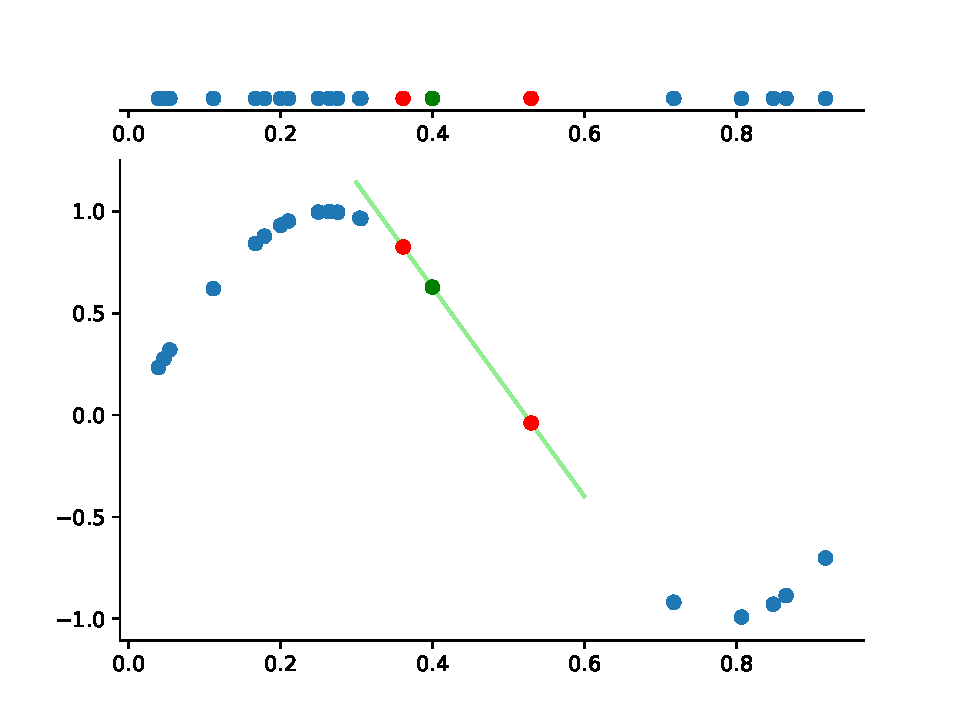
\includegraphics[width=\linewidth]{images/vis1d.pdf}
		\caption{A one-dimensional example of linear interpolation}
		\label{fig:one-dim-interpolation}
	\end{subfigure}%
	~ 
	\begin{subfigure}[t]{0.5\textwidth}
		\centering
		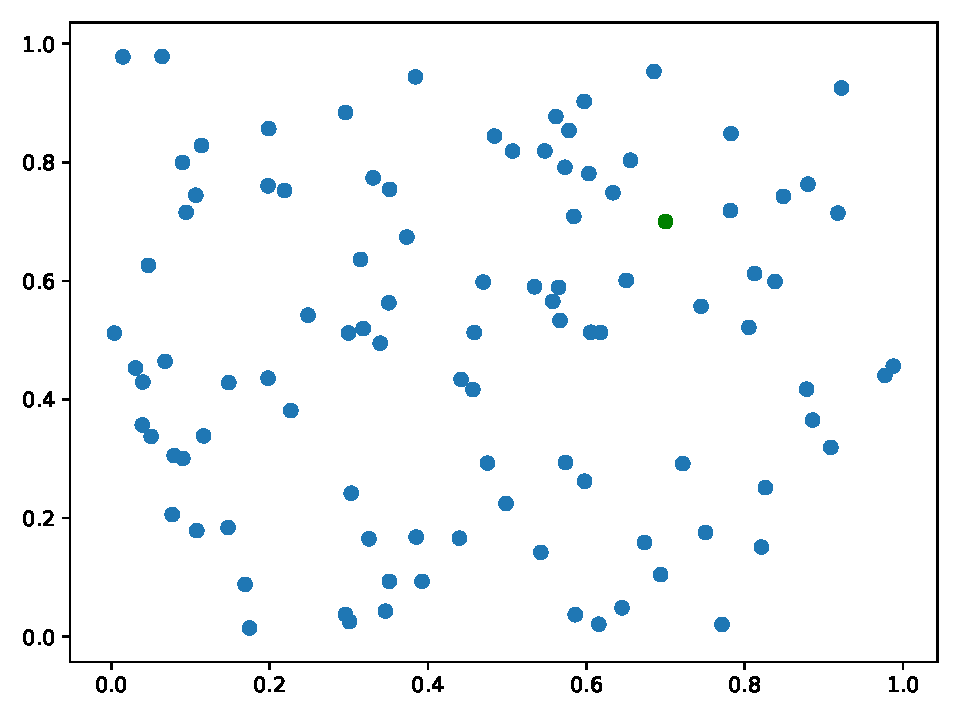
\includegraphics[width=\linewidth]{images/vis2d1.pdf}
		\caption{A set of two-dimensional datapoints}
		\label{fig:3dinterpolate-1}
	\end{subfigure}
	\caption{}
	
\end{figure}

In two dimensions things get more complicated as we now have a set of points with $X$ and $Y$ coordinates (Figure \ref{fig:3dinterpolate-1}). One fast way to find the closest points to the point that should be interpolated is using Delaunay triangulation. This is a method to separate the space between the points into triangles while trying to maximize their smallest angle and to make sure no other point is inside the circumcircle of the triangles\footcite{Delaunay}. Connecting the centers of the circumcircles results in a Voronoi diagram.  

Afterwards, the closest three points can be found very quickly by checking the nodes of the surrounding triangle  (Figure \ref{fig:3dinterpolate-2}). If we now again have a function $f(X,Y)$ similar to the one-dimensional example, we can create a unique plain through the three points and get the interpolated value for any pair of $X$ and $Y$ on this layer. (Figure \ref{fig:3dinterpolate-3})


\begin{figure}[] % also temporary
	\centering
	\begin{subfigure}[t]{0.48\textwidth}
		\centering
		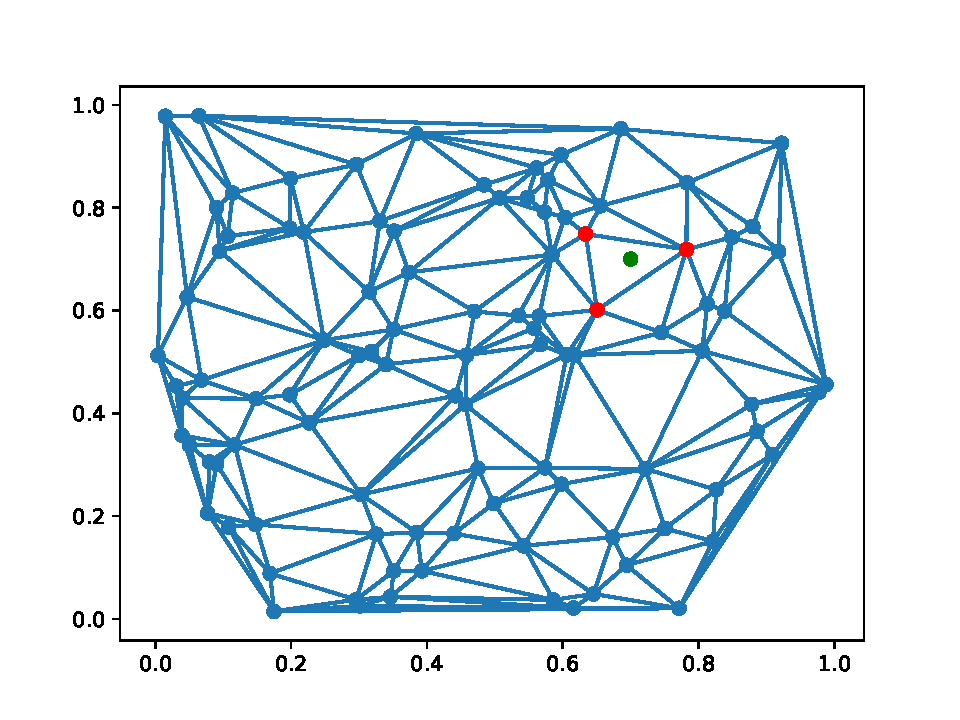
\includegraphics[width=\linewidth]{images/vis2d2.pdf}
		\caption{A Delaunay triangulation of the points from Figure~\ref{fig:3dinterpolate-1}}
	\label{fig:3dinterpolate-2}
	\end{subfigure}%
	~ 
	\begin{subfigure}[t]{0.48\textwidth}
		\centering
		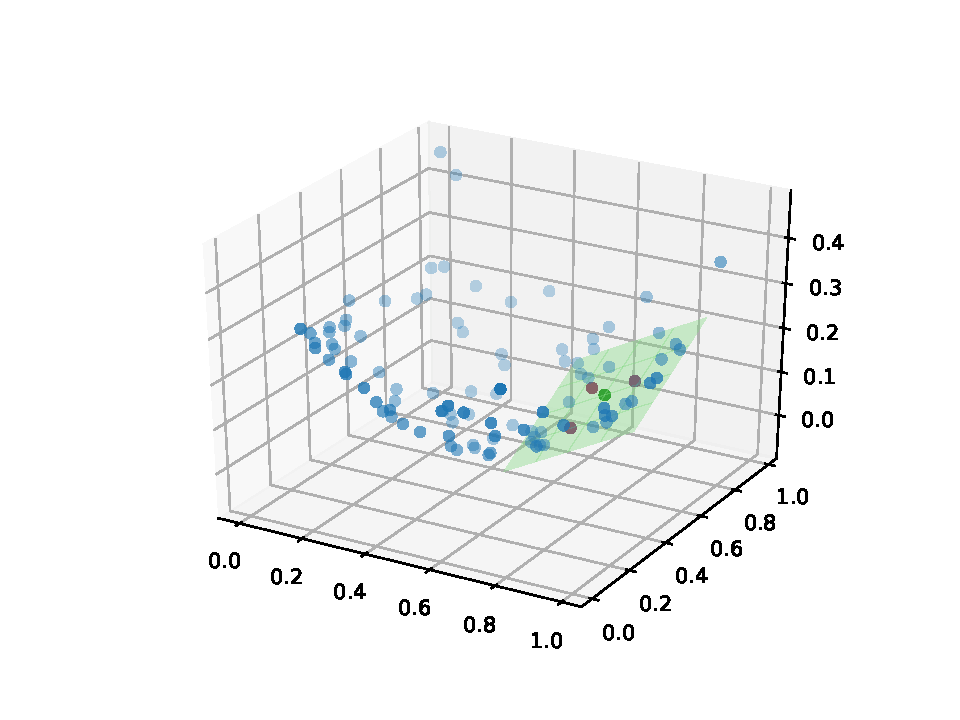
\includegraphics[width=\linewidth]{images/vis2d3.pdf}
		\caption{A $f(X,Y)$ interpolated via the green plane}
		\label{fig:3dinterpolate-3}
	\end{subfigure}
	\caption{}

\end{figure}



This approach has the advantage that it can be extended in more than two dimensions by replacing the triangle in the Delaunay triangulation with an n-simplex in n dimensions. The \texttt{scipy.spatial.Delaunay} python function allows to quickly calculate it thanks to the \texttt{Qhull} library\footnote{\url{http://www.qhull.org/}}. One noticeable limitation of this method is that data can't be extrapolated. Therefore, the possible output is limited to the convex hull of the input parameter space (as seen in Figure \ref{fig:3dinterpolate-2}).

\subsection{Implementation}
\label{sec:griddata-implementation}
For doing the actual interpolations, the \texttt{scipy.interpolate.griddata} function is used with the \texttt{method="linear"} argument which itself uses \texttt{scipy.interpolate.LinearNDInterpolator} to do an interpolation similar to the one described above. The function is given a $6\times n$ matrix of the six parameters and an $n$-sized list of the water retention fraction for those $n$ simulations. In addition, \texttt{griddata} supports not only calculating interpolations for one set of parameters, but also for lists of parameters which allows to quickly generate 2d diagrams as seen in  Figure \ref{fig:griddataresults}.

\subsection{Results}

Most notable about the results of the griddata interpolation (see Figure \ref{fig:griddataresults}) are the many fine details that can be seen. This is mostly caused by the fact that this method only uses the closest values for interpolations and therefore there is no smoothing. These details might just be random derivations of the simulation and not a higher resolution of the data. Another thing that can be seen in the bottom right corner of Figure \ref{fig:griddata1} is that griddata can't extrapolate data.

\begin{figure}[h!] % also temporary
	\centering
	\begin{subfigure}[t]{0.5\textwidth}
		\centering
		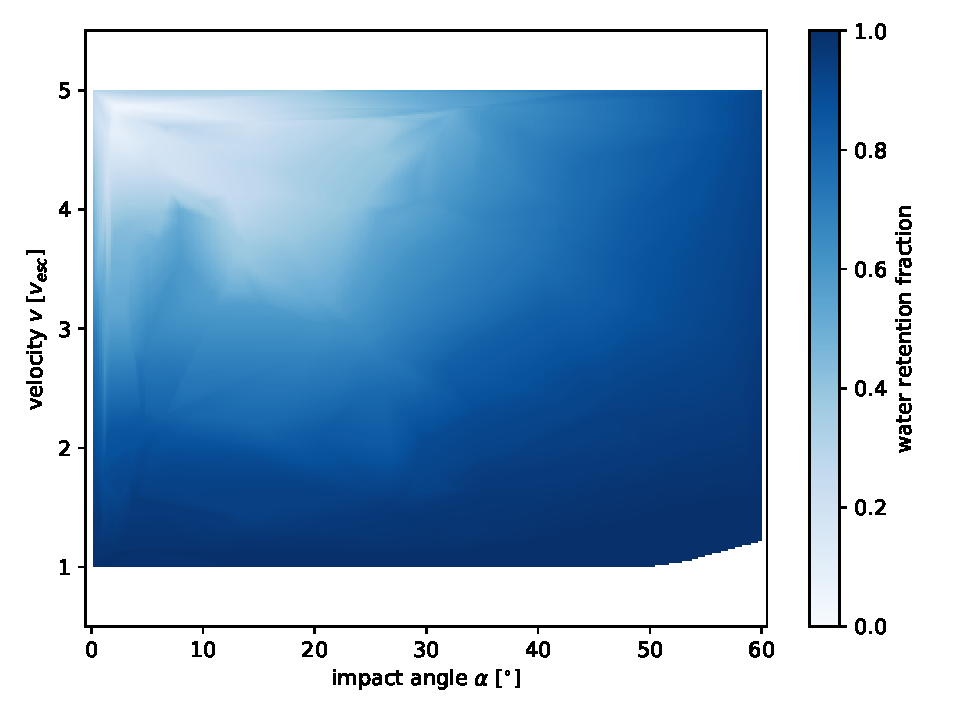
\includegraphics[width=\linewidth]{images/plots/griddata1.pdf}
		\caption{$m_{total}=\num{e22}$, $\gamma=0.6$, $wt=wp=0.15$}
		\label{fig:griddata1}
	\end{subfigure}%
	~ 
	\begin{subfigure}[t]{0.5\textwidth}
		\centering
		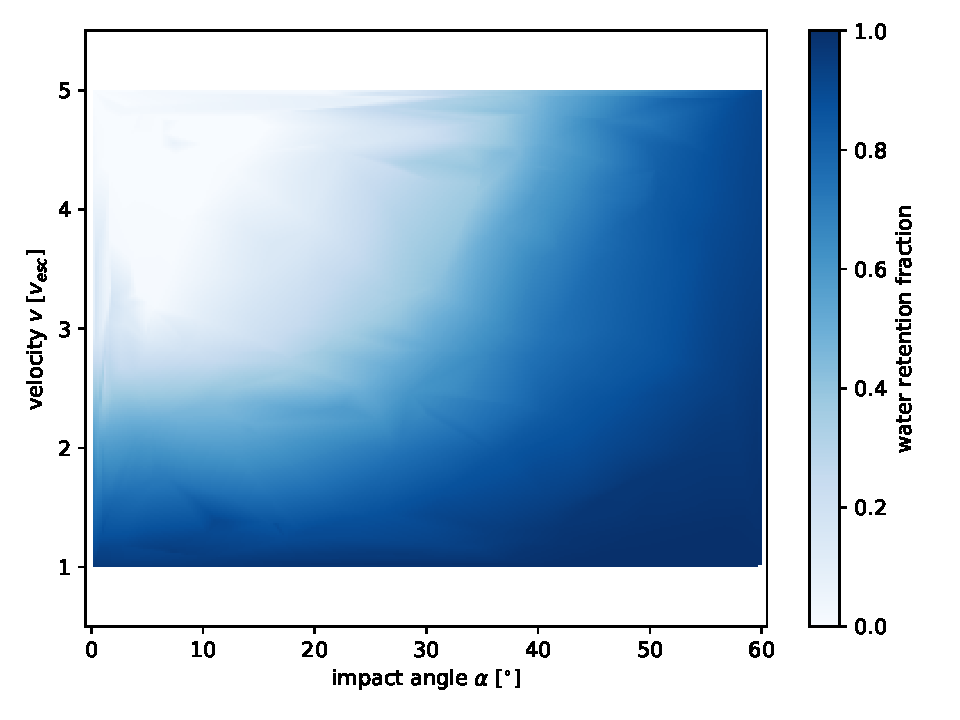
\includegraphics[width=\linewidth]{images/plots/griddata2.pdf}
		\caption{$m_{total}=\num{e24}$, $\gamma=0.6$, $wt=wp=0.15$}
		\label{fig:griddata2}
	\end{subfigure}
	\caption{Interpolation result using griddata}
	\label{fig:griddataresults}
\end{figure}


\section{RBF interpolation}

\subsection{Theory}

Another approach to interpolate data is using \textit{Radial Basis Functions}. A very good explanation on how they work is given in \cite{RBF} which is shortly summarized below:

 A function $\phi$ for which $\phi(x)=\phi(\left\|x\right\|)$ is true is called \textit{radial}. Now to be able to interpolate, we need to find the interpolation function $s(x)$ which is the same as the given values $p_i$ in all points.

\begin{align}
	s(x_i)=p_i,\quad i=1,2,\dots,n
\end{align}

The RBF interpolation now consists of a linear combination of $\phi(\left\|x-x_i\right\|)$ for a chosen radial function $\phi$ which $n$ constants $\lambda_i$.

\begin{align}
	s(x)&=	\sum_{i=1}^{n}\lambda_i\phi(\left\|x-x_i\right\|) \\
	%
	p_j&=\sum_{i=1}^{n}\lambda_i\phi(\left\|x_j-x_i\right\|),\quad j=1,2,\dots,n
\end{align}

Therefore this can be written as a linear matrix equation:

\begin{align}
	\begin{bmatrix}
		\phi(\left\|x_1-x_1\right\|) & \phi(\left\|x_2-x_1\right\|) & \dots  & \phi(\left\|x_n-x_1\right\|) \\
		\phi(\left\|x_1-x_2\right\|) & \phi(\left\|x_2-x_2\right\|) & \dots  & \phi(\left\|x_n-x_2\right\|) \\
		\vdots                       & \vdots                       & \ddots & \vdots                       \\
		\phi(\left\|x_1-x_n\right\|) & \phi(\left\|x_2-x_n\right\|) & \dots  & \phi(\left\|x_n-x_n\right\|)
	\end{bmatrix} 
	\begin{bmatrix}
		\lambda_1 \\
		\lambda_2 \\
		\vdots    \\
		\lambda_n
	\end{bmatrix}
	=
	\begin{bmatrix}
		p_1    \\
		p_2    \\
		\vdots \\
		p_n
	\end{bmatrix}
\end{align}
or simply
\begin{align}
	\Phi\lambda=p
\end{align}

with $\Phi$ being a symmetric $n \times n $ matrix as $\left\|x_j-x_i\right\|=\left\|x_i-x_j\right\|$. There are many possibilities for the radial basis function $\phi(r)$. It can be for example linear ($r$), gaussian ($e^{-r^2}$) or multiquadric ($\sqrt{\left(\frac{r}{\epsilon}\right)^2 + 1}$) with $\epsilon$ being a constant that defaults to the approximate average distance between nodes.

As an example, consider the three points $x_1=0$, $x_1=3$ and $x_1=5$ with $p(x_1)=0.2$, $p(x_2)=0.8$ and $p(x_3)=0.1$ and choose the gaussian RB-function\todo{looks odd} we get the following:
\begin{align}
	\begin{bmatrix}
		\phi(0) & \phi(3)  & \phi(5) \\
		\phi(3) & \phi(0) & \phi(2) \\
		\phi(5) & \phi(2)  & \phi(0)
	\end{bmatrix} 
	\lambda
	=
		\begin{bmatrix}
			1              & \num{1.23e-4} & \num{1.39e-11} \\
			\num{1.23e-4}  & 1             & \num{1.83e-2}  \\
			\num{1.39e-11} & \num{1.83e-2} & 1
		\end{bmatrix} 
	\begin{bmatrix}
\lambda_1 \\
\lambda_2 \\
\lambda_3
\end{bmatrix}
=
\begin{bmatrix}
0.22\\0.8\\0.1
\end{bmatrix}
\end{align}

Solving this linear matrix equation using \texttt{numpy.linalg.solve} gives us the solution for $\lambda$:
\begin{equation}
	\lambda=\begin{bmatrix}
	0.200 \\0.798  \\0.085
	\end{bmatrix}
\end{equation}

Combined we get the following linear combination for the interpolated function $s(x)$:
\begin{equation}
	s(x)=0.200\phi(\left\|x\right\|)+
		0.798\phi(\left\|x-3\right\|)+
		0.085\phi(\left\|x-5\right\|)
\end{equation}



\begin{figure}[h] % also temporary
	\centering
	\begin{subfigure}[t]{0.5\textwidth}
		\centering
		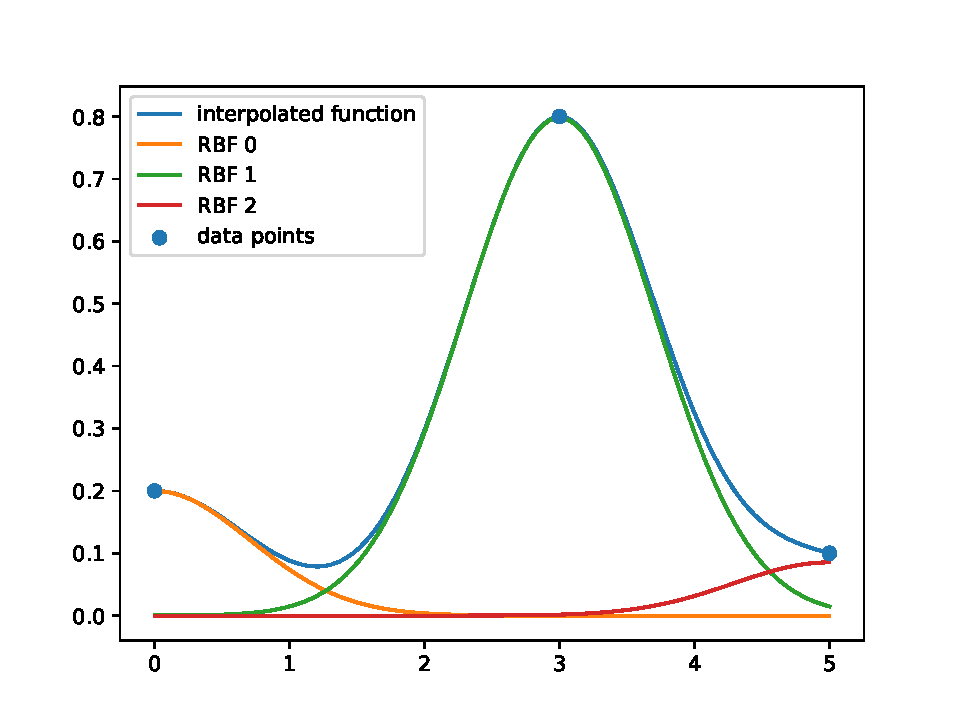
\includegraphics[width=\linewidth]{images/rbf1.pdf}
		\caption{Lorem ipsum}
		\label{fig:rbf-1}
	\end{subfigure}%
	~ 
	\begin{subfigure}[t]{0.5\textwidth}
		\centering
		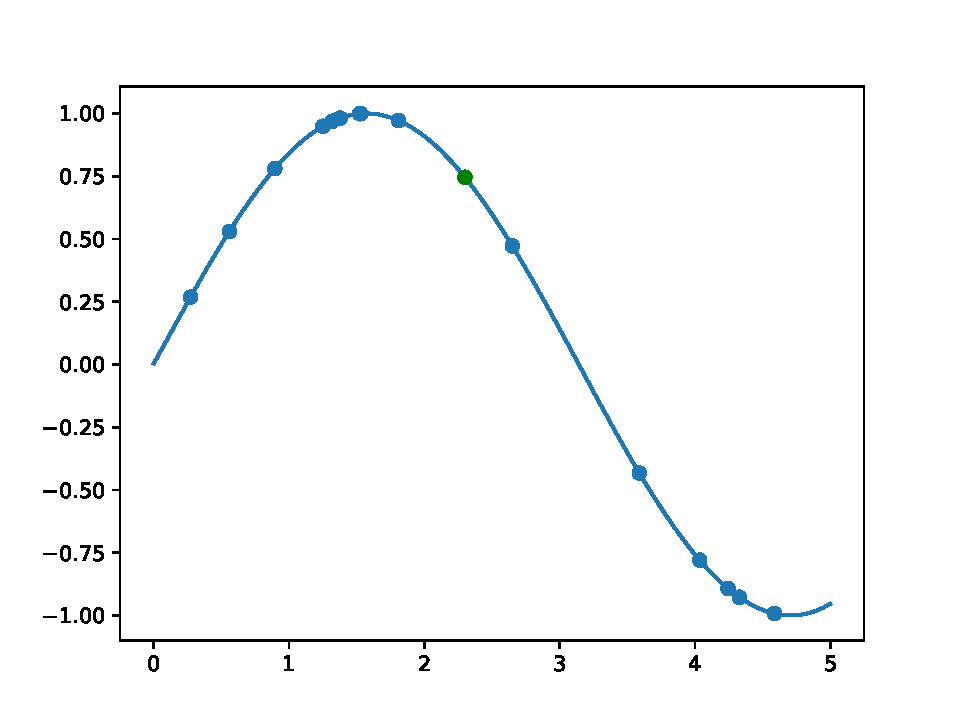
\includegraphics[width=\linewidth]{images/rbf2.pdf}
		\caption{Lorem ipsum, lorem ipsum,Lorem ipsum, lorem ipsum,Lorem ipsum}
		\label{fig:rbf-2}
	\end{subfigure}
	\caption{Caption place holder}
	
\end{figure}

Applying the same method to a list of random points allows to interpolate their values for arbitrary other points like the green point on the sinus-like curve in Figure \ref{fig:rbf-2}. This can also be trivially extended in $m$ dimensions by replacing $x$ with an $x\in\mathbb{R}^m$ and using a norm in $\mathbb{R}^m$ for $\left\|\ \right\|$.

\subsection{Implementation}

The scipy function \texttt{scipy.interpolate.Rbf} allows directly interpolating a value similar to \texttt{griddata} in Section \ref{sec:griddata-implementation}. A difference in usage is that it only allows interpolating a single value, but as it is pretty quick it is possible to calculate multiple values sequentially.

\subsection{Results}

% !TeX spellcheck = en_US
\begin{figure}[h] % also temporary
	\centering
	\begin{subfigure}[t]{0.5\textwidth}
		\centering
		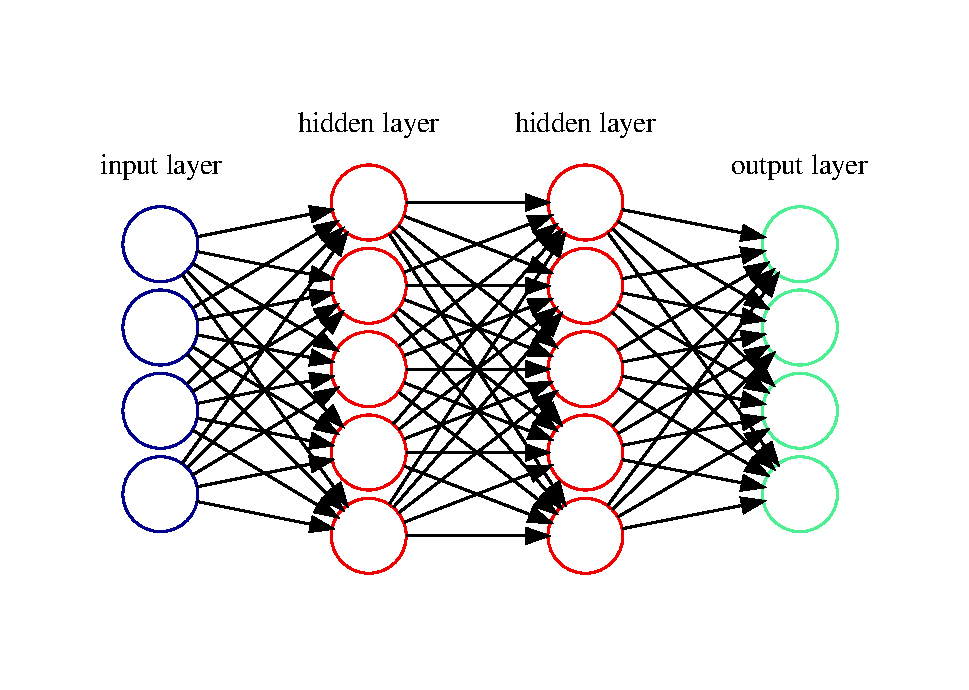
\includegraphics[width=\linewidth]{images/graphviz/general.pdf}
		\caption{An example for a neural network}
		\label{fig:neuralnetwork-general}
	\end{subfigure}%
	~ 
	\begin{subfigure}[t]{0.5\textwidth}
		\centering
		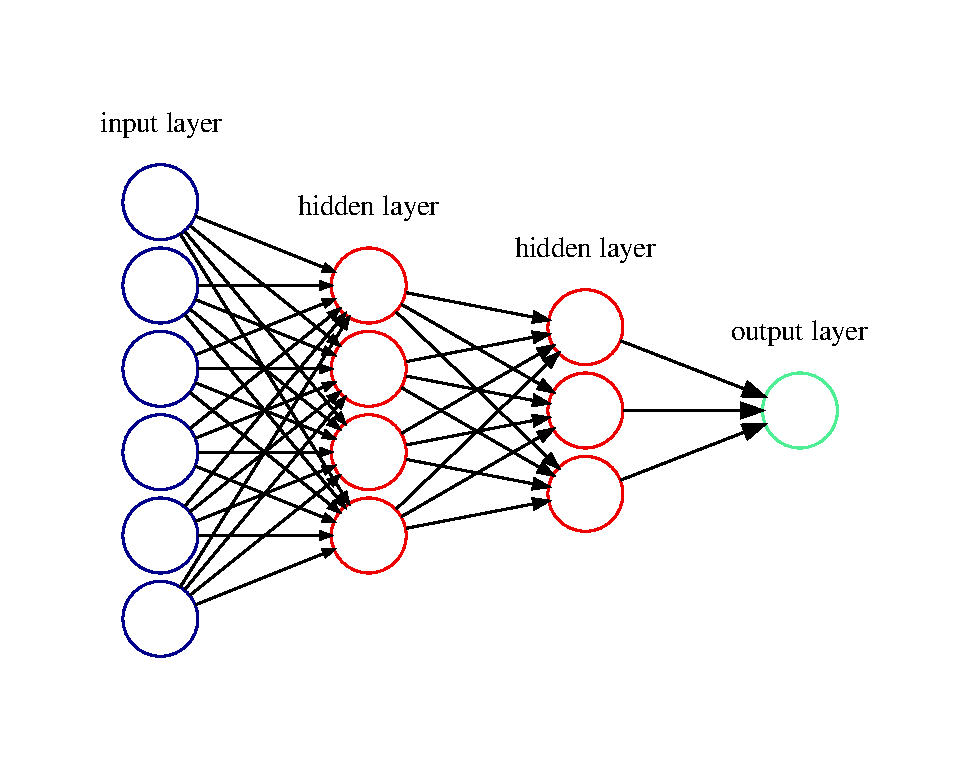
\includegraphics[width=\linewidth]{images/graphviz/graph.pdf}
		\caption{The network used for interpolation}
		\label{fig:neuralnetwork-graph}
	\end{subfigure}
	\caption{}
	
\end{figure}

\section{Artificial Neural Networks}

Another method that is good at taking pairs of input and output values and then able to predict output values for arbitrary input sets is using \textit{Artificial neural networks} (\texttt{ANNs}).

\subsection{Theory}

The idea behind artificial neural networks is trying to emulate the functionality of neurons by having nodes that are connected to each others. The weights $w$ of these connections are modified during the training to represent the training data and can then be used to predict new results for input values not seen in the training data.

Every neural network needs an input layer with as many nodes as input parameters and an output layer with a node for every output value. In between, there can be multiple hidden layers with an arbitrary amount of nodes. (Figure \ref{fig:neuralnetwork-general})

If we first only consider a single neuron, then on every iteration it calculates the sum over all input values multiplied with their weight $w$. Afterwards, an activation function $g$ is applied to the sum $z$ to get the prediction $\hat{y}$.

\begin{equation}
	z=\sum_{i}w_ix_i \qquad \hat{y}=g(z)
\end{equation}

The non-linear activation function allows the network to be able to approximate all types of functions instead of being just a linear function itself. Popular activation functions are the sigmoid function $\sigma(x)={\frac {1}{1+e^{-x}}}$ and the ReLU function (\textit{rectified linear unit}, $f(x)=\max(0,x)$).\footcite{NN-math}

After this first step (the \textit{feedforward}) is done, the weights can be modified by comparing the prediction with the real output (the \textit{backpropagation}). The function that describes the error between them is called the Loss function and one possible form is the mean squared error function:

\begin{equation}
	L(\hat{y},y)=\sum_{i}(\hat{y}_i-y_i)^2
\end{equation}

To update the weights, the derivative of the Loss function with respect to the weights is calculated and added to the existing weights.\todo{more details?}\footcite{NN-python}

\subsection{Implementation}

As building a neural network from scratch gets complex very quickly, it is easier to use \texttt{Keras}\footnote{\url{https://keras.io}} which provides easy to use high-level functions over the calculations provided by \texttt{TensorFlow}\footnote{\url{https://www.tensorflow.org/}}. To build our network, we only need to specify the structure of the layers, take our input and let the network train for 200 epochs (iterations of feedforward and backpropagation). 

The network needs six nodes in the input layer for the input parameters and one node in the output layer for the prediction. In between, are two layers with decreasing numbers of nodes as this seems to give the best results. (Figure \ref{fig:neuralnetwork-graph})

\begin{lstlisting}[language=Python,caption=The used model as Keras code,label=lst:model]
from keras import Sequential
from keras.layers import Dense

model = Sequential()
model.add(Dense(6, input_dim=6, activation='relu'))
model.add(Dense(4, kernel_initializer='normal', activation='relu'))
model.add(Dense(3, kernel_initializer='normal', activation='relu'))
model.add(Dense(1, kernel_initializer='normal', activation="sigmoid"))
model.compile(loss='mean_squared_error', optimizer='adam')

model.fit(x, Y, epochs=200, validation_data=(x_test, Y_test))

\end{lstlisting}

\subsection{Training}

To find the ideal parameters to use, the simulation data (excluding the data from Section \ref{sec:comparison}) is split into two groups: The complete original set of simulations and \SI{80}{\percent} of the new simulation set is used to train the neural network while the remaining \SI{20}{\percent} are used for validation. This means that after every epoch the loss function is not only calculated for the training data, but also for the separate validation data (Figure \ref{fig:loss_val}). Finally, the model with the lowest loss on the validation data set was chosen (Listing \ref{lst:model}).


\begin{figure}[h] % also temporary
	\centering
	\begin{subfigure}[t]{0.5\textwidth}
		\centering
		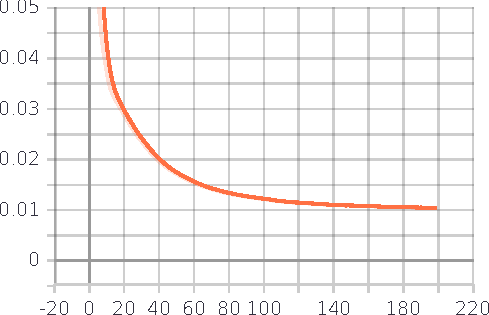
\includegraphics[width=\linewidth]{images/loss.pdf}
		\caption{loss function on the training data}
		\label{fig:loss}
	\end{subfigure}%
	~ 
	\begin{subfigure}[t]{0.5\textwidth}
		\centering
		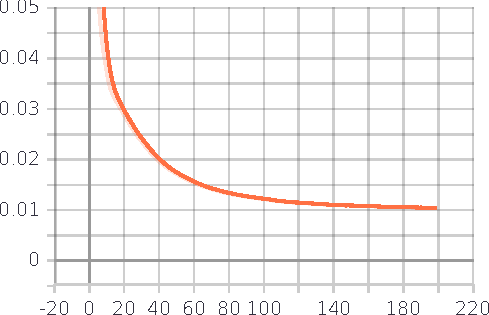
\includegraphics[width=\linewidth]{images/val_loss.pdf}
		\caption{loss function on the validation data}
		\label{fig:val_loss}
	\end{subfigure}
	\caption{During training the loss function (mean squared error) decreases with every epoch until it converges to a final value.}
	\label{fig:loss_val}
	
\end{figure}

After the training, the resulting model is saved in a small \texttt{HDF5} file which can be used to evaluate the model very quickly (about \SI{100}{\milli\second} for \num{10000} interpolations).


\subsection{Results}

Figure \ref{fig:nnresults} \todo{text}

\begin{figure}[h!] % also temporary
	\centering
	\begin{subfigure}[t]{0.5\textwidth}
		\centering
		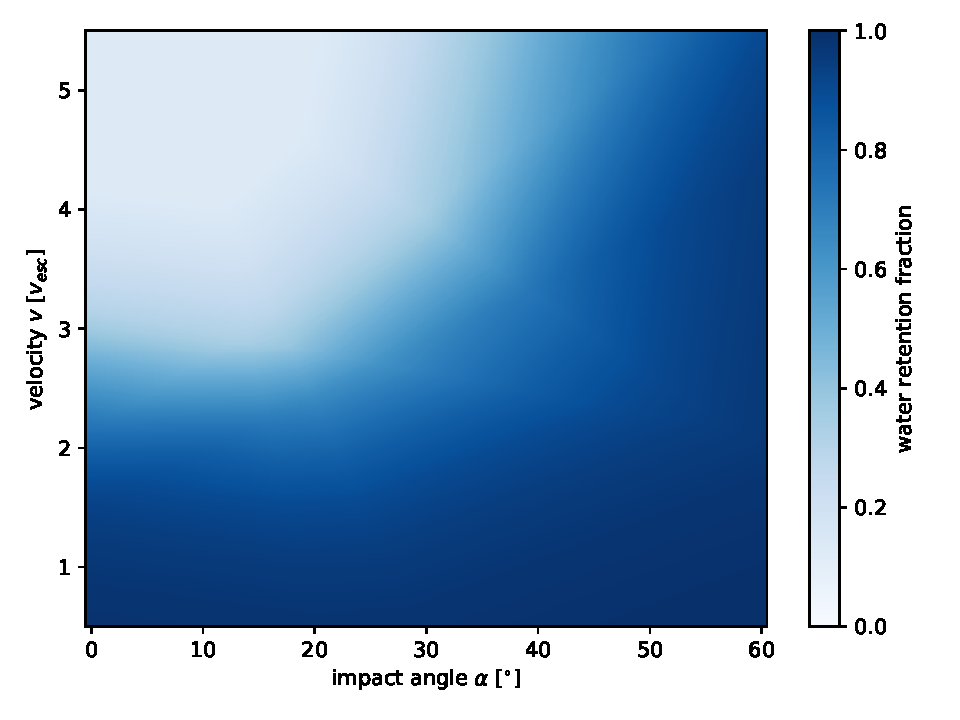
\includegraphics[width=\linewidth]{images/plots/nn1.pdf}
		\caption{$m_{total}=\num{e22}$, $\gamma=0.6$, $wt=wp=0.15$}
		\label{fig:nn1}
	\end{subfigure}%
	~ 
	\begin{subfigure}[t]{0.5\textwidth}
		\centering
		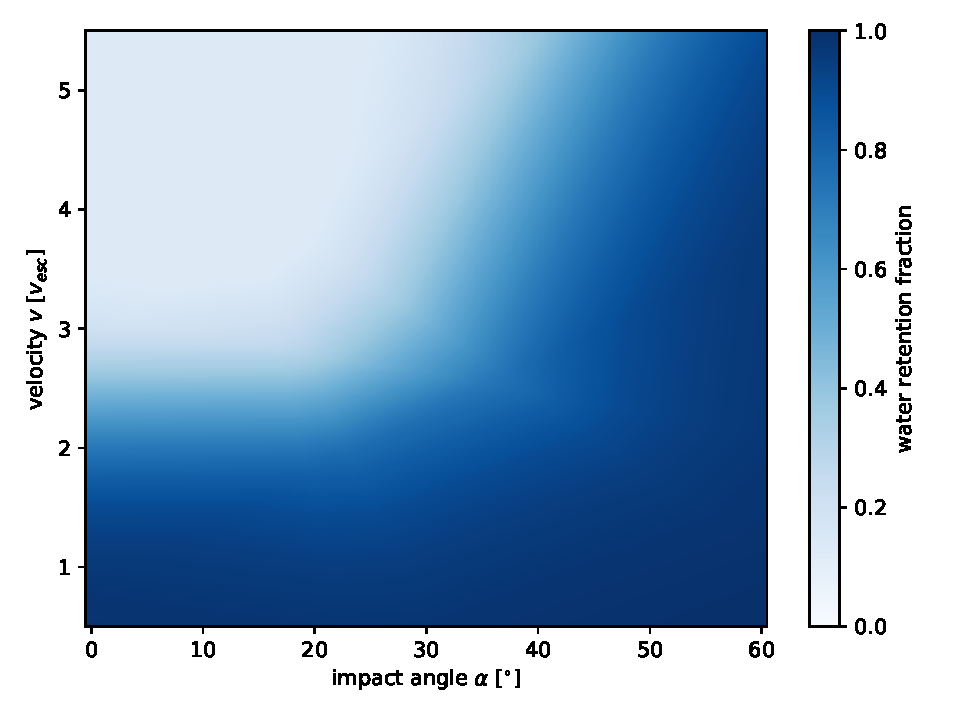
\includegraphics[width=\linewidth]{images/plots/nn2.pdf}
		\caption{$m_{total}=\num{e24}$, $\gamma=0.6$, $wt=wp=0.15$}
		\label{fig:nn2}
	\end{subfigure}
	\caption{Interpolation result using the trained neural network}
	\label{fig:nnresults}
\end{figure}


% !TeX spellcheck = en_US
\section{Comparison}

To compare the three methods explained above and measure their accuracy an additional set of 100 simulations (with the same properties as the ones listed in Section \ref{sec:resimulation}). These results are neither used to train or select the neural network, nor are in the dataset for griddata and RBF interpolation. Therefore we can use them to generate predictions for their parameters and compare them with the real fraction of water that remained in those simulations. By taking the mean absolute difference or the mean squared error between the predictions and the real result the accuracy of the different methods can be estimated (Table \ref{tab:comparison}). As one of these parameter sets is outside the convex hull of the training data and griddata can't extrapolate, this simulation is skipped and only the remaining 99 simulations are considered for the griddata accuracy calculation. 

Of the three methods, the trained neural network has the highest mean squared error. This seems to be\todo{more interpretations}

Another important aspect to compare is the interpolation speed. The neural network is able to give the 100 results in about \SI{4}{\milli\second} (after loading the trained model). RBF interpolation is still reasonably fast taking about \SI{8.5}{\second} (\SI{85}{\milli\second} per interpolation). But as \texttt{griddata} expects a grid-based parameter space, it becomes really slow when adding the resimulation data with random parameters. A single interpolation takes about \SI{35}{\second} totaling to around an hour for all 99 test cases. Using only the original dataset brings the runtime down to around \SI{10}{\second}, but causes the results to be less accurate than all other methods.

\begin{table}
	\centering
	\begin{tabular}{rcc}
		                              & {mean squared error} & {mean error} \\
		griddata (only original data) &        0.014         &    0.070     \\
		               neural network &        0.010         &    0.069     \\
		                          RBF &        0.008         &    0.057     \\
		                     griddata &        0.005         &    0.046
	\end{tabular}
	\caption{prediction accuracy for the different interpolation methods}
	\label{tab:comparison}
\end{table}

% !TeX spellcheck = en_US
\chapter{Comparison and Conclusion}
\label{sec:comparison}

To compare the three methods explained above and measure their accuracy an additional set of 100 simulations (with the same properties as the ones listed in Section \ref{sec:resimulation}) was created. These results are neither used to train or select the neural network, nor are in the dataset for griddata and RBF interpolation. Therefore, we can use them to generate predictions for their parameters and compare them with the real fraction of water that remained in those simulations. By taking the mean absolute difference and the mean squared error between the predictions and the real result, the accuracy of the different methods can be estimated (Table \ref{tab:comparison}). As one of these parameter sets is outside the convex hull of the training data and griddata can't extrapolate, this simulation is skipped and only the remaining 99 simulations are considered for the griddata accuracy calculation. 

Of the three methods, the trained neural network has the highest mean squared error. This seems to be at least partly caused by the fact that during training the neural network, the data is generalized, causing the final network to output the \enquote{smoothest} interpolations. While this causes the errors to be higher, it might be possible that the fine structured details in the simulation output is just a artifact of the simulation setup and doesn't represent real world collisions.
\todo{better wording}

Another important aspect to compare is the interpolation speed. The neural network is able to give the 100 results in about \SI{4}{\milli\second} (after loading the trained model). RBF interpolation is still reasonably fast, taking about \SI{8.5}{\second} (\SI{85}{\milli\second} per interpolation). But as \texttt{griddata} expects a grid-based parameter space, it becomes really slow when adding the resimulation data with random parameters. A single interpolation takes about \SI{35}{\second} totaling to around an hour for all 99 test cases. Using only the original dataset brings the runtime down to around \SI{10}{\second}, but causes the results to be less accurate than all other methods. (first row in Table \ref{tab:comparison})

\begin{table}[h]
	\centering
	\begin{tabular}{rcc}
		                              & {mean squared error} & {mean error} \\
		griddata (only original data) &        0.014         &    0.070     \\
		               neural network &        0.010         &    0.069     \\
		                          RBF &        0.008         &    0.057     \\
		                     griddata &        0.005         &    0.046
	\end{tabular}
	\caption{Prediction accuracy for the different interpolation methods}
	\label{tab:comparison}
\end{table}

\appendix

\chapter{Mass retention}

While this thesis focuses on the water retention after the collisions, the same methods can be applied to the fraction of basalt from the core of the two bodies that remains after the collision.


\begin{table}
	\centering
	\begin{tabular}{rcc}
		& {mean squared error} & {mean error} \\
		neural network &        0.043         &    0.167     \\
		RBF &        0.032         &    0.149     \\
		griddata &        0.041         &   0.169
	\end{tabular}
	\caption{prediction accuracy for the different interpolation methods}
	\label{tab:mass_comparison}
\end{table}

\begin{figure}
	\centering
	\begin{subfigure}[t]{0.5\textwidth}
		\centering
		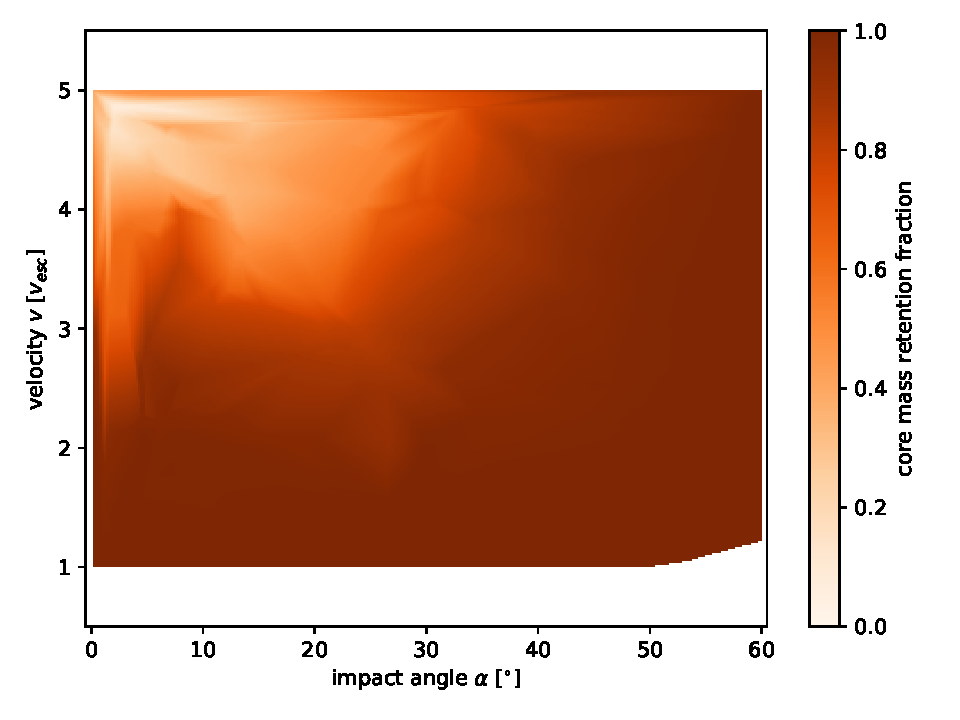
\includegraphics[width=\linewidth]{images/plots/mass_griddata1.pdf}
		\caption{Griddata with $m_{total}=\num{e22}$}
		\label{fig:mass_griddata1}
	\end{subfigure}%
	~ 
	\begin{subfigure}[t]{0.5\textwidth}
		\centering
		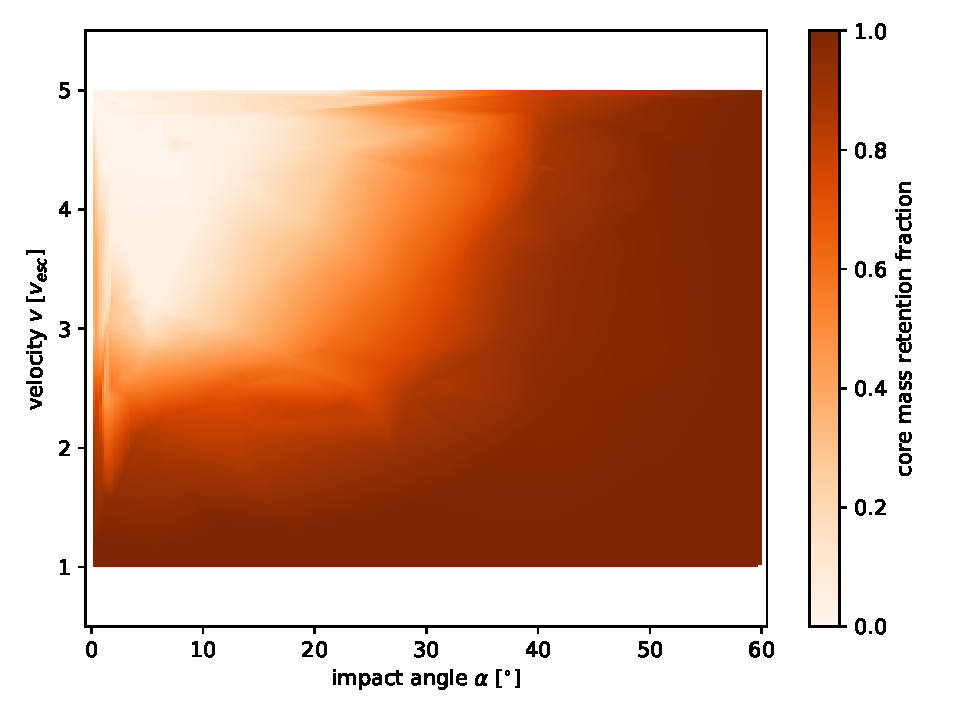
\includegraphics[width=\linewidth]{images/plots/mass_griddata2.pdf}
		\caption{Griddata with $m_{total}=\num{e24}$}
		\label{fig:mass_griddata2}
	\end{subfigure}
~ 
	\begin{subfigure}[t]{0.5\textwidth}
	\centering
	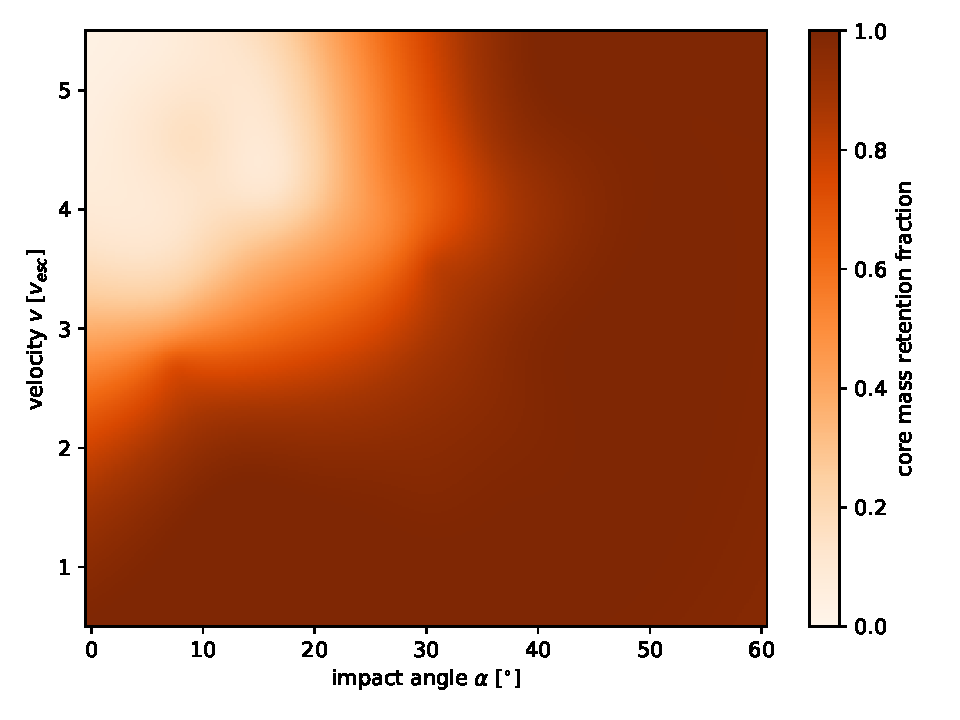
\includegraphics[width=\linewidth]{images/plots/mass_rbf1.pdf}
	\caption{RBF with $m_{total}=\num{e22}$}
	\label{fig:mass_rbf1}
\end{subfigure}%
~ 
\begin{subfigure}[t]{0.5\textwidth}
	\centering
	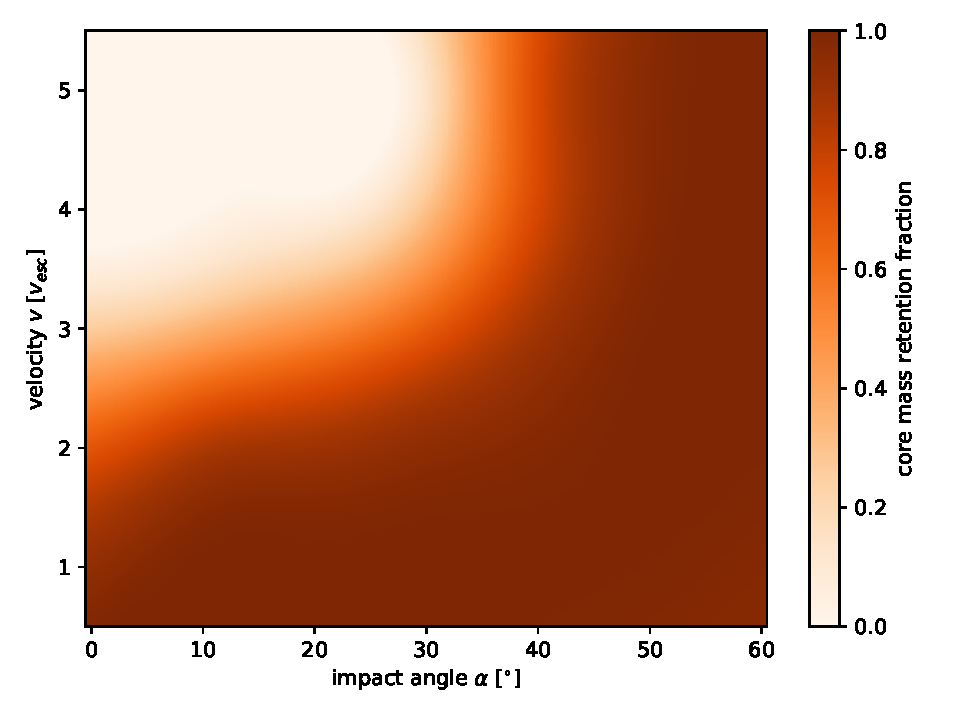
\includegraphics[width=\linewidth]{images/plots/mass_rbf2.pdf}
	\caption{RBF with $m_{total}=\num{e24}$}
	\label{fig:mass_rbf2}
\end{subfigure}
~ 
\begin{subfigure}[t]{0.5\textwidth}
	\centering
	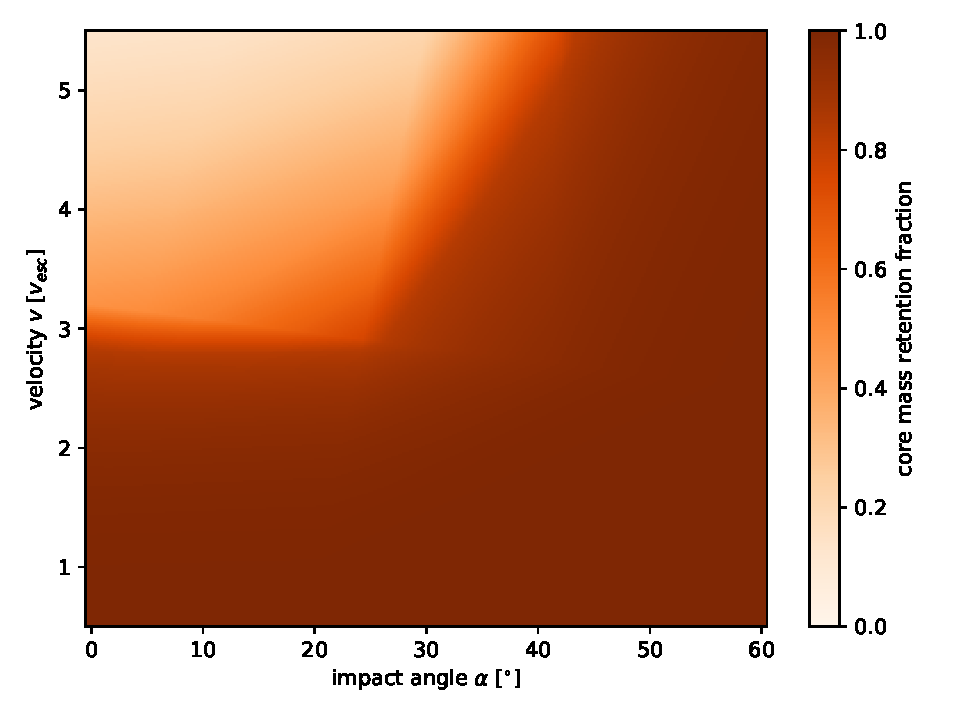
\includegraphics[width=\linewidth]{images/plots/mass_nn1.pdf}
	\caption{Neural Network  with $m_{total}=\num{e22}$}
	\label{fig:mass_nn1}
\end{subfigure}%
~ 
\begin{subfigure}[t]{0.5\textwidth}
	\centering
	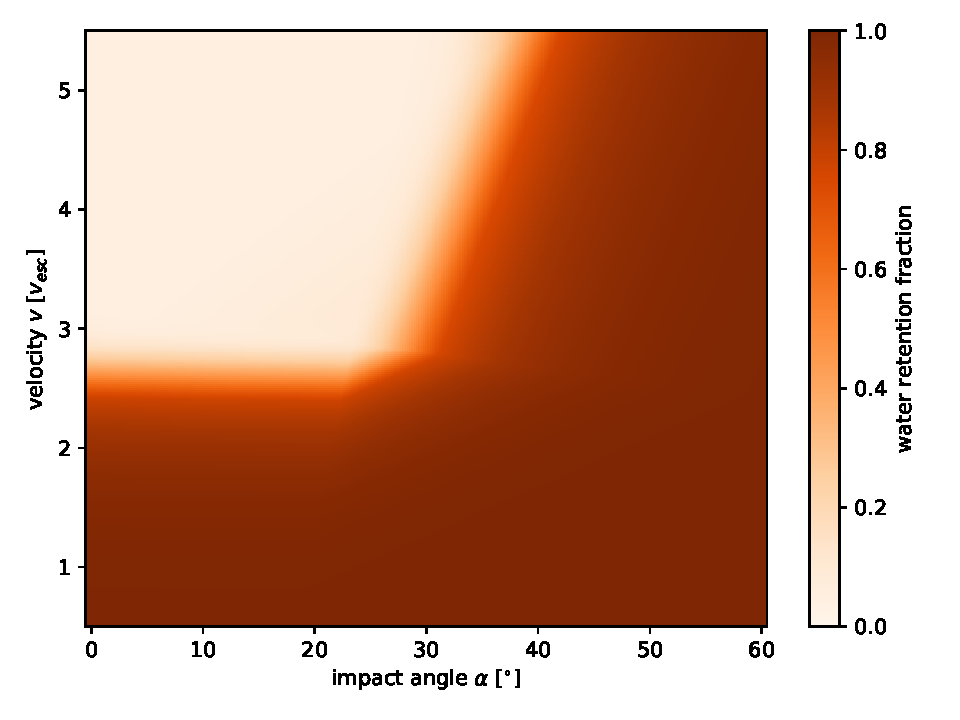
\includegraphics[width=\linewidth]{images/plots/mass_nn2.pdf}
	\caption{Neural Network  with $m_{total}=\num{e24}$}
	\label{fig:mass_nn2}
\end{subfigure}
	\caption{TODO}
	\label{fig:mass_results}
\end{figure}




\chapter{Other TODOs}

\todo[inline]{All captions should start with an uppercase letter and end with a .}


\printbibliography


\end{document}

